
\section{Theorie}
\label{sec:Theorie}

Unter dem Begriff Zeeman-Effekt wird ein Phänomen verstanden, welches Auftritt, wenn ein Atom in ein Magnetfeld gebracht wird. Aufgund der verschiedenen magnetischen Momente der Zustände des Atoms mit gleichem Energieniveau ohne anglegten Magnetfeld, kommt es im Magnetfeld zu einer Aufspaltung dieser Energieniveaus. Diese Aufspaltung wird im Spektrum in Form zusätzlicher Wellenlängen sichtbar. Von besonderer Bedeutung für diesen Effekt ist der aus Spin und Drehimpuls der Elektronen in verschiedenen Zuständen zusammengesetzte Gesamtdrehimpuls sowie der zugehörige Landé-Faktor.


\subsection{Drehimpuls, Spin und magnetisches Moment eines Elektrons}
Elektronen in der Elektronenhülle des Atoms kann sowohl ein Drehimpuls als auch Spin zugeordnet werden. Die Quantenzahlen $n$, $l$ und $s$ der Eigenzustände des Elektrons haben folgende Beziehung zu den Drehimpuls $\vec{l}$ und Spin $\vec{s}$:
\begin{align*}
	|\vec{l}|= \hbar \sqrt{l(l+1)} & \text{ mit } l=0, 1, \hdots, n-1\\
	|\vec{s}|= \hbar \sqrt{s(s+1)} & \text{ mit } s=\frac{1}{2}.
\end{align*}
Daraus ergibt sich das magnetische Moment zu:
\begin{gather*}
	\vec{\mu}_l=-\mu_\text{B} \frac{\vec{l}}{\hbar}=-\mu_\text{B} \sqrt{l(l+1)} \vec{l}_e \\
	\vec{\mu}_s=- g_\text{s} \mu_\text{B} \frac{\vec{s}}{\hbar}=- g_\text{s} \mu_\text{B} \sqrt{s(s+1)} \vec{s}_e
\end{gather*}
wobei es sich bei $\vec{l}_e$ und $\vec{s}_e$ um die jeweiligen Einheitsvektoren und bei $\mu_\text{B}=\frac{e_0 \hbar}{2 m_0}$ um das Bohrsche Magneton handelt. Die Größe $e_0$ ist die Ladung des Elektrons und $m_0$ die Masse. Die Größe $g_\text{s}$ ist der Landé-Faktor des Elektrons und is gilt $g_\text{s} \approx 2$. Dieser Unterschied beim Spin zum Bahndrehimpuls wird als magnetomechanische Anomalie des Elektrons bezeichnet und folgt aus der Dirac-Gleichung. Das Gesamte magnetische Moment ist dann durch:
\begin{gather*}
	\vec{\mu}_\text{ges}= \vec{\mu}_l+\vec{\mu}_s
\end{gather*}
gegeben.

\subsection{Kopplung von Drehimpuls und Spin zum Gesamtdrehimpuls}

Wie die Drehimpulse und Spins in einem Mehrelektronensystem zum Gesamtdrehimpuls koppeln ist von System zu System verschieden und nur schwer zu behandeln. Es können jedoch zwei wichtige Grenzfälle relativ einfach behandelt werden. Der eine Grenzfall ist die LS- oder auch Russell-Saunders-Kopplung. Dies ist der Grenzfall für Atome mit kleiner Kernladungszahl. Hierbei setzen sich die die Drehimpulse und Spins jeweils sich zu einem Drehimpuls \[\vec{L}=\sum_i \vec{l}_i\] und einem Spin \[\vec{S}=\sum_i \vec{s}_i\] der gesammten Elektronenhülle zusammen. Der Drehimpuls und Spin wird dabei durch die Drehimpulse und Spins in den unabgeschlossenen Schalen zusammengesetzt, da sich diese in den abgeschlossenen Schalen gegenseitig aufheben. Der Gesamtdrehimpuls der Elektronenhülle ergibt sich zu \[\vec{J}=\vec{L}+\vec{S}.\] Für die jeweiligen magnetischen Momente gilt:
\begin{gather*}
	\vec{\mu}_L=-  \mu_\text{B} \frac{\vec{L}}{\hbar}=- \mu_\text{B} \sqrt{L(L+1)} \vec{L}_e\\
	\vec{\mu}_S=- g_\text{s} \mu_\text{B} \frac{\vec{S}}{\hbar}=- g_\text{s} \mu_\text{B} \sqrt{S(S+1)} \vec{S}_e\\
	\vec{\mu}_J=\vec{\mu}_L+\vec{\mu}_S.
\end{gather*}

Der andere Grenzfall wird als $j-j$-Kopplung bezeichnet. Bei dies ist der Grenzfall für Atome mit hoher Kernladungszahl.



\subsection{Aufspaltung im Magnetfeld}
\begin{figure}
	\centering
	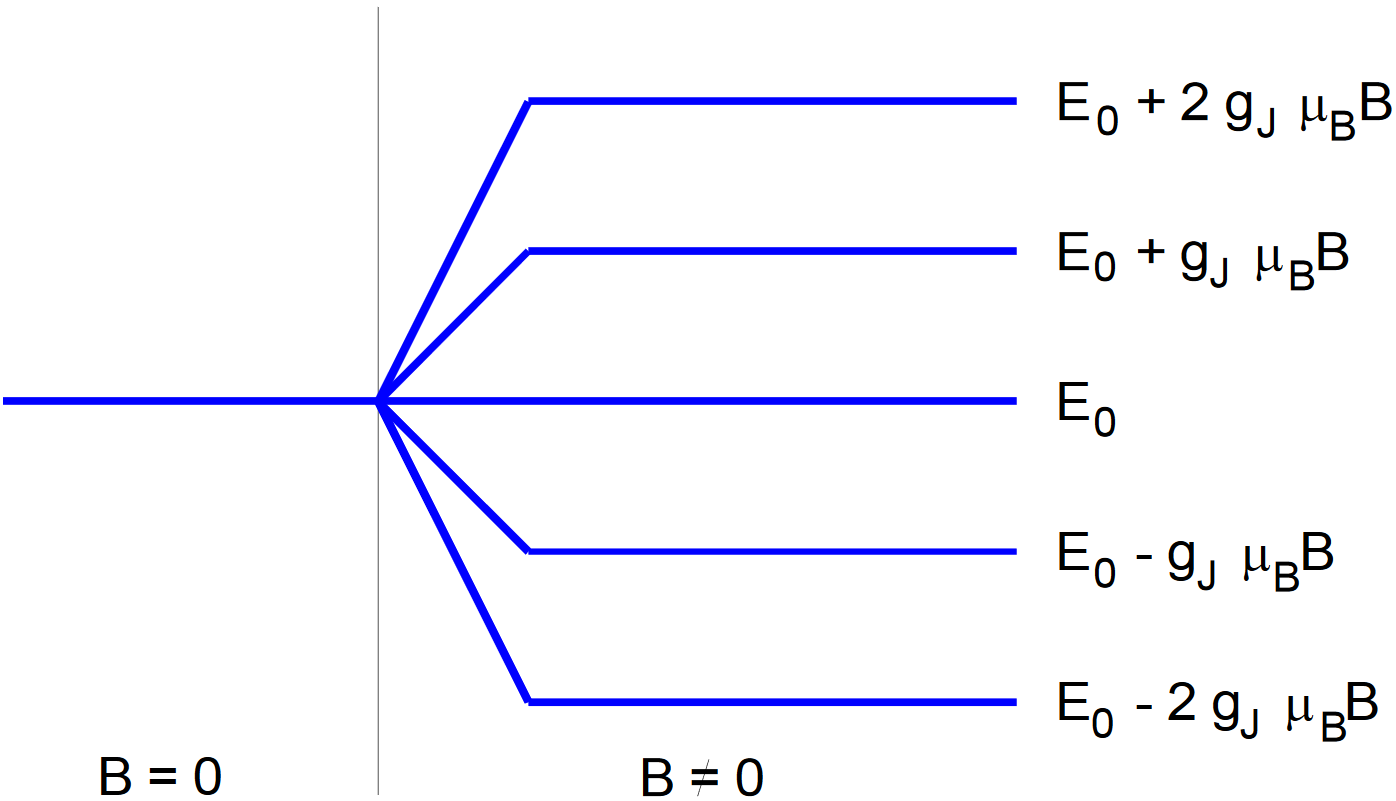
\includegraphics[width=\linewidth-250pt,height=\textheight-250pt,keepaspectratio]{content/Images/generelleAufspaltung.png}
    \caption{Theoretische Aufspaltung eines Enegieniveaus eines Atoms mit $J=2$ im Magnetfeld \cite{V27}.}
    \label{fig:aborb}
\end{figure}
